\subsection*{ Angular velocity control}

In the previous chapter has been discussed how the control demand is calculated through two, with different nature, controllers. This torque demand is used to give the desired angular velocity reference for the wheels and thus the torque that will be fed back to the satellite as seen in the \cite{block diagram}. The output torque from the linear and non-linear controllers has three elements which has to be transformed in the tetrahedron configuration using the matrix \eqref{transmatrix}.  A \textit{PI} controller has been designed to control the angular velocity of the motor as seen in the \figref{fig:blockdi222}:
%\begin{figure}[H]
%	\centering
%	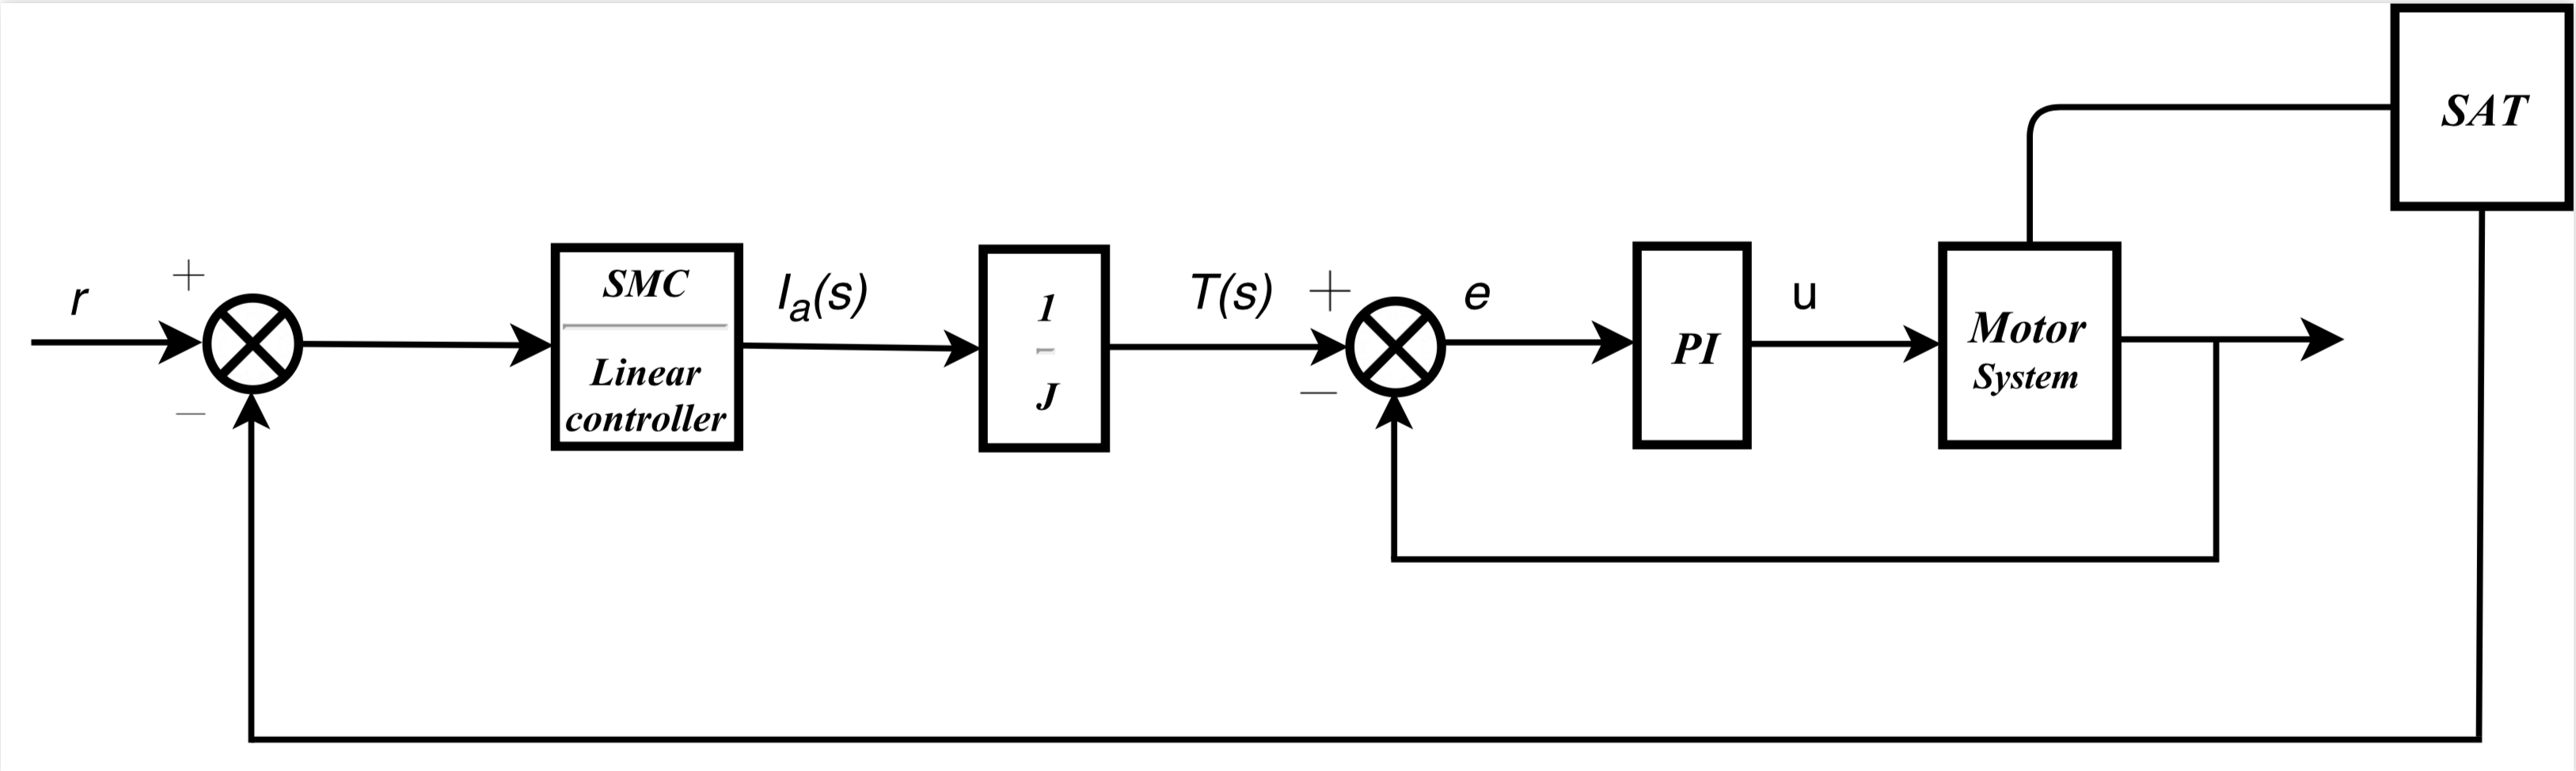
\includegraphics[width=1.0\linewidth]{figures/block_diagram_2}
%	\caption{Block diagram of the motor control with PID controller}
%	\label{fig:blockdi222}
%\end{figure}  
%
The PI controller gains are chosen by trial and error in order to achieve faster closed loop response, settling time less than 1 $s$ zero steady state error and asymptotically stable system. The gains are chosen to be:   
%
\begin{flalign*}
	k_{p} = 0.006 \\ k_{i} = 6
\end{flalign*}


The root locus of one motor with PI controller is seen in the \figref{fig:rlocus33}

\begin{figure}[H]
	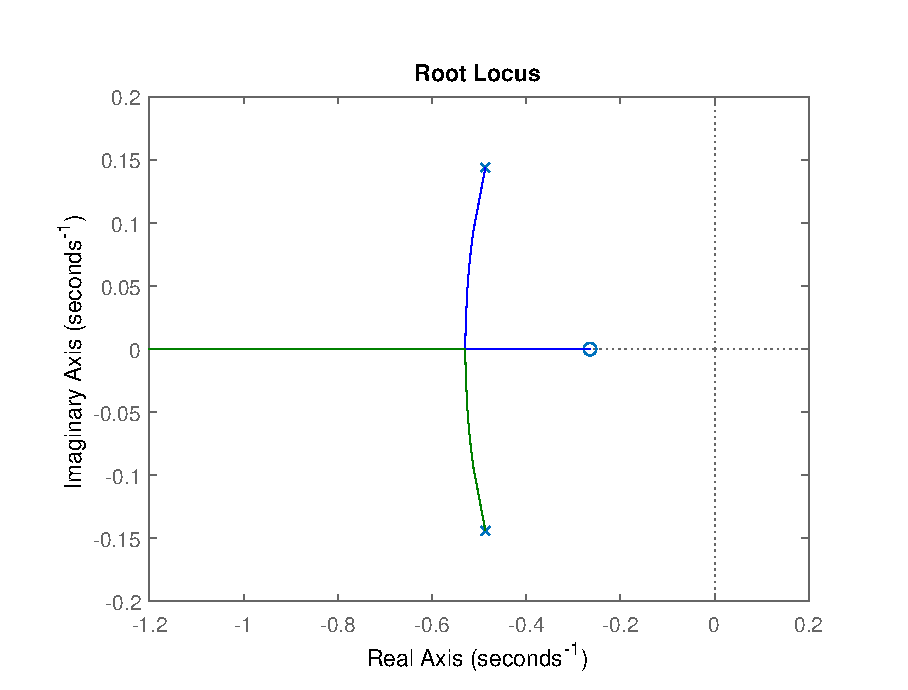
\includegraphics[width=0.9\linewidth]{figures/pid_rootlocus}
	\caption{Root locus of one motor with PI controller}
	\label{fig:rlocus33}
\end{figure}
Furthermore in the \figref{fig:rlocus44}  it can be seen how the poles of the closed loop system are moving to the right half plane, by setting the gain $k_{p}$ to 0, and thus causing saturation of the motor(it is depicted the original without zoom in to the left and with zoom in to the right )
\begin{table}[H]
	\begin{minipage}[b]{0.49\linewidth}
		\centering
		\begin{figure}[H]
			\centering
			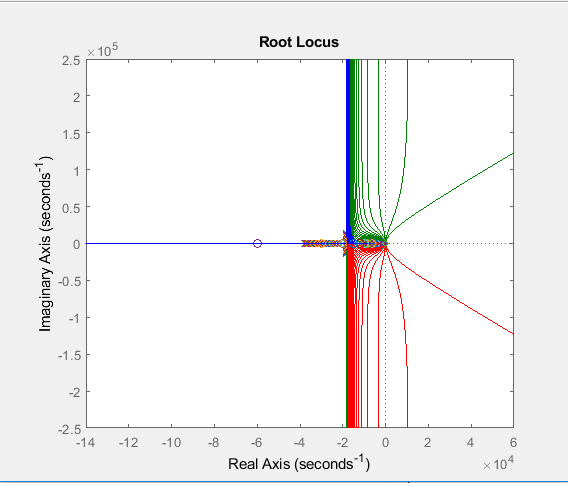
\includegraphics[width=1\linewidth]{figures/pid_saturate3}
			%\caption{ Electrical and mechanical part of the motor }
			%	\label{fig:electromech}
		\end{figure}
	\end{minipage}\hfill
	\begin{minipage}[b]{0.49\linewidth}
		\centering
		\begin{figure}[H]
			\centering
			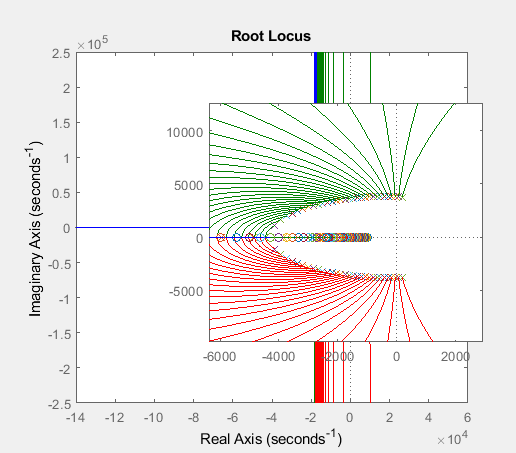
\includegraphics[width=1\linewidth]{figures/pid_saturate2}
			%\caption{Mechanical part of the motor}
			%\label{fig:distancecontrol4}
		\end{figure}
	\end{minipage}
	\caption{ Root locus of one motor in saturation }
	\label{fig:rlocus44}
\end{table}
